\section{Theory}
\subsection{Fourier}

\subsection{The dB-scale}

\subsection{Smoothing}

\subsection{Zero padding}

\subsection{Windowing}

\subsection{Energy}

\section{Using build-in Matlab functions}
Hvilke funktioner anvendes?
Skalering?
Korrekte frekvensbins?

\section{Frequency analysis}
\subsection{Car engine}

\begin{figure}
	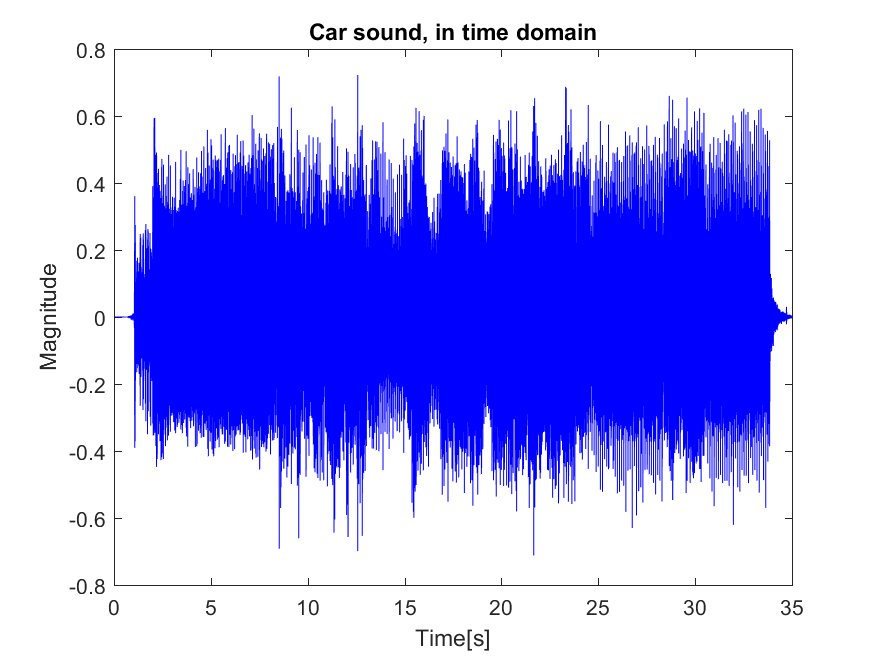
\includegraphics[width=\textwidth]{code/Car_figure1.png}
	\caption{kage}
\end{figure}

\subsubsection{DFT}

\subsubsection{Analysis}

\subsubsection{Conclusion}

\subsection{Noise from a windmill}
\subsubsection{DFT}

\subsubsection{Analysis}

\subsubsection{Conclusion}

\subsection{EKG}
\subsubsection{DFT}

\subsubsection{Analysis}

\subsubsection{Conclusion}

\subsection{Breaking wine glass}
\subsubsection{DFT}

\subsubsection{Analysis}

\subsubsection{Conclusion}

\subsection{Music}
\subsubsection{DFT}

\subsubsection{Analysis}

\paragraph{Genre 1}

\paragraph{Genre 2}

\paragraph{Genre 3}

\paragraph{Genre 4}

\subsubsection{Conclusion}

\section{Further analysis of signals}
Eksperimenter med udglatning, zero-padding og windowing 

\section{Energy}

\section{Discussion}

\section{Conclusion}